The user should expect to input desired commands, controls, and specific
settings such as temperature and length of time by a easily accessible
touchscreen. The touchscreen will be attached to a Raspberry Pi that will handle
communications between the user and the various sensors and heating elements.
The user can expect that whichever temperature they set for their desired
application, that the temperature will remain constant.

\subsection{Touchscreen Control System}

\subsubsection{Description}
The user needs a way to be able to input commands and specific settings before
starting the beer brewing process. This will be done by attaching a touchscreen
to a Raspberry Pi 4. The Raspberry Pi will then communicate with the automated
brewing system through a webserver that is hosted by the various
microcontrollers that manage various sensors. 

\subsubsection{Source}
This requirement came from Dr. Chris Conly. He requested that our team have a
method by which the user can interface with the automated brewing system and
input various commands, controls, and recipe specific settings.
\subsubsection{Priority}
This feature is of \textbf{Critical} priority. Without this feature the user
would be unable to make the automated brewing system produce the user's desired results. 

\subsection{Programmable HLT Heating Element Temperature Management}
\subsubsection{Description}

The heating element on the HLT will need to maintain the temperature that is set
by the user via the main control touchscreen. The reason for customizable temperature is due to the varying
temperature requirements set by the recipe chose by the user. This temperature control will
managed by an ESP32 microcontroller. The temperature of the vessel will be
monitor by a DS18B20 digital thermometer. The microcontroller will take
continuous readings from the thermometer. When it begins dropping below the
desire temperature the microcontroller will send a signal to a mosfet. When the
mosfet receives that signal it switch states and allow for power to be delivered
to the heating element. Once the desired temperature is reached, the
microcontroller will send another signal to the mosfet. The mosfet will then
turn off, and this would turn off the power to the heating element.

\begin{figure}[H]
	\centering
	\graphicspath{.\images}
	\fbox{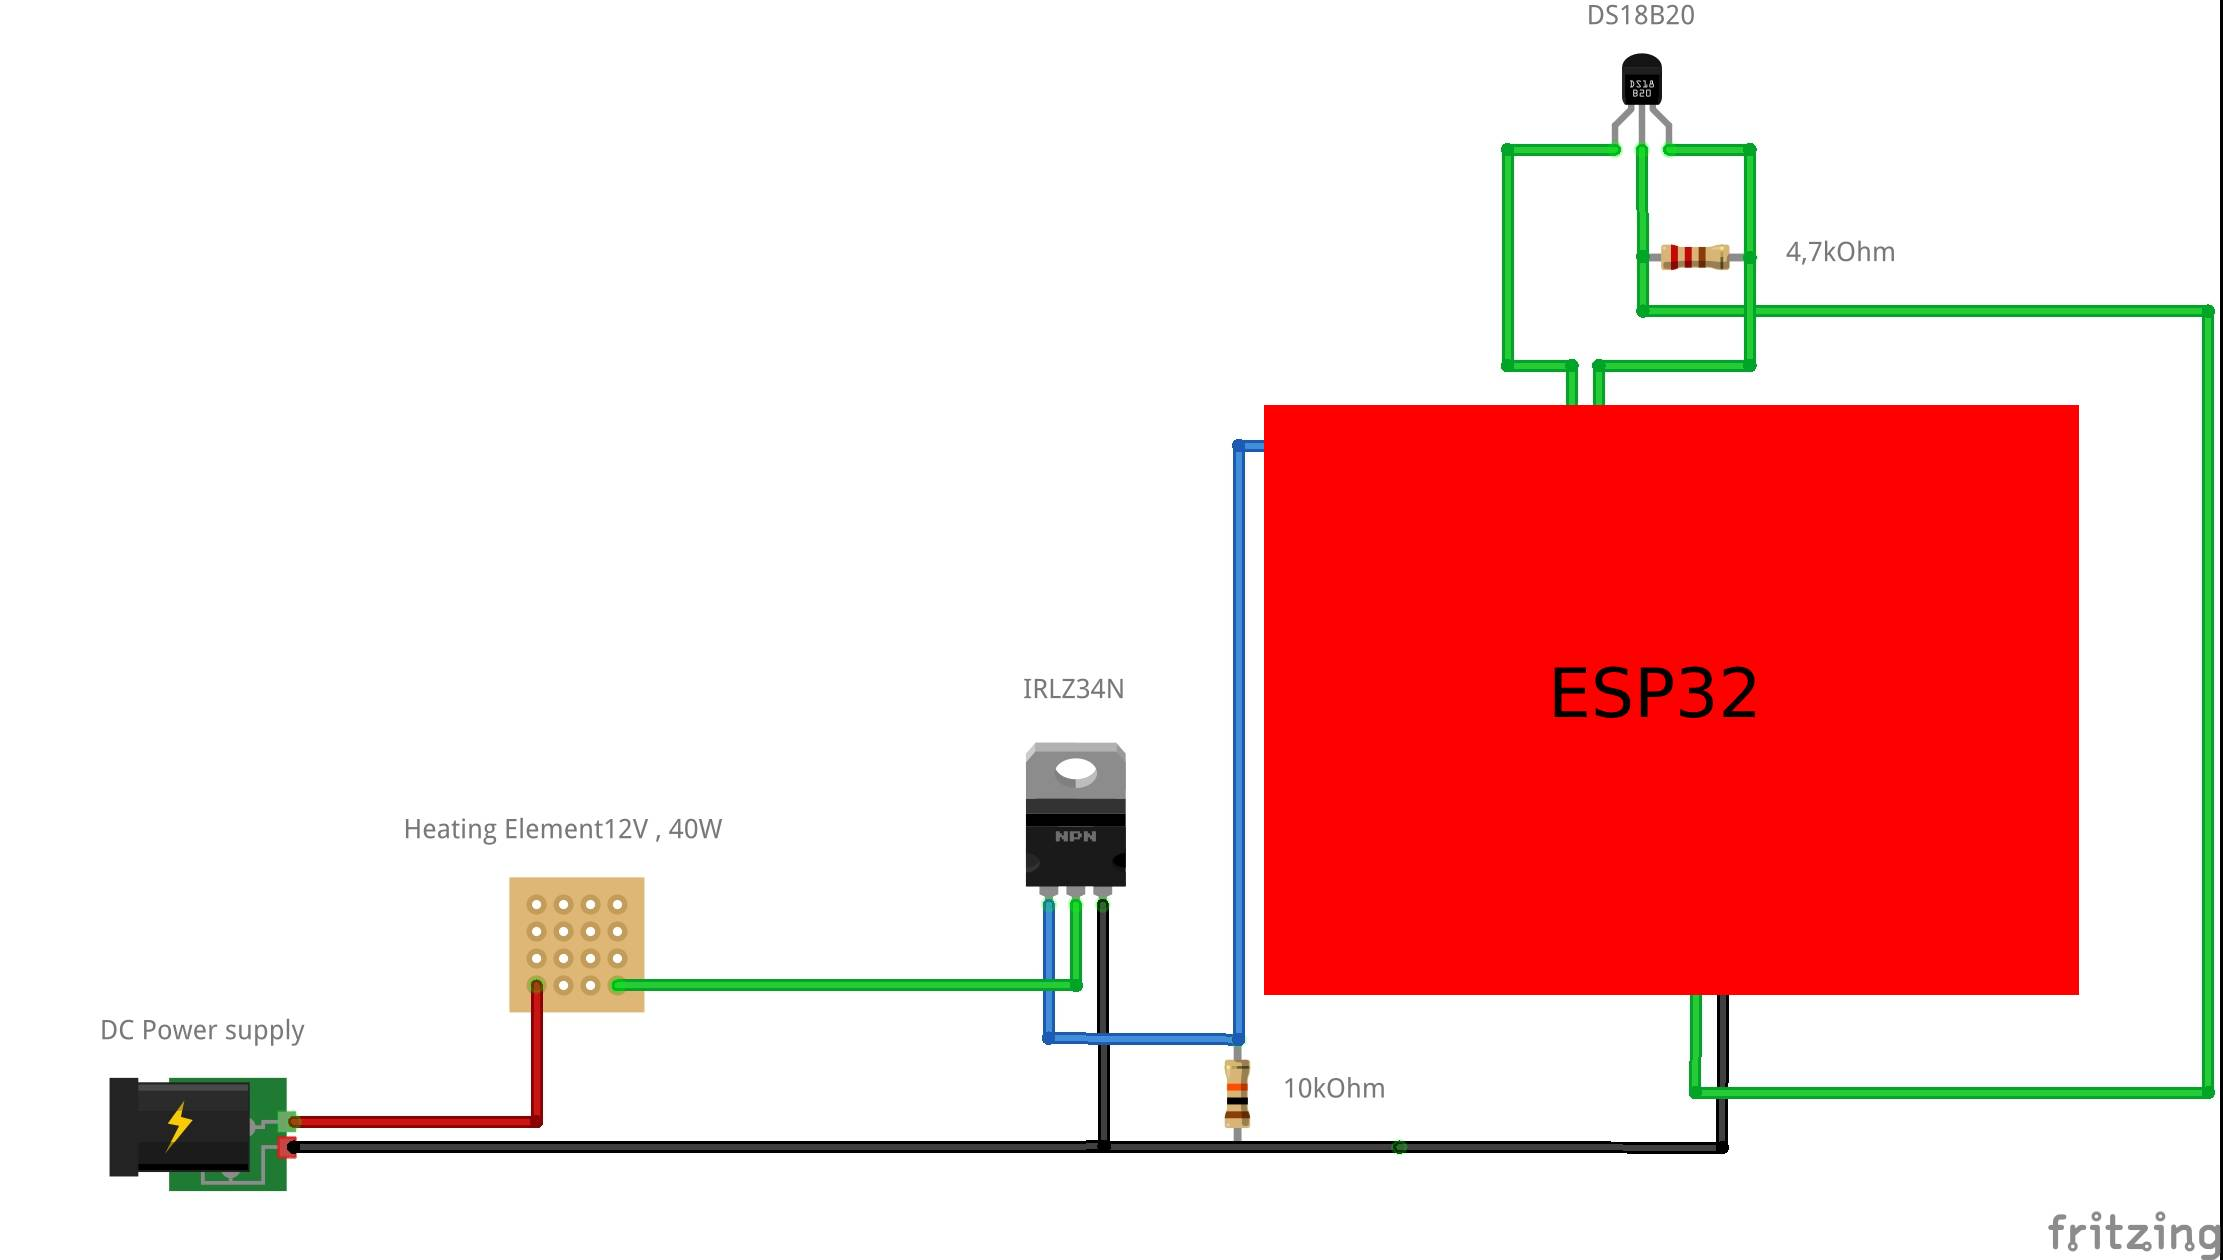
\includegraphics[scale=0.5]{images/temperature_control_diagram.jpg}}
	\caption{HLT Temperature Controller Diagram}
\end{figure}

\subsubsection{Source}
This requirement came from Dr. Chris Conly. He requested that our team enable
the user to be able to set a specific temperature via the main control
touchscreen. The water is to stay at a constant boiling temperature to maximize
effectiveness of the mashing process.  
\subsubsection{Standards}
\begin{itemize}
\item IEC 60730
\item IEC 60335
\item EN ISO 13849
\end{itemize}
\subsubsection{Priority}
This feature is of \textbf{Critical} priority. Without this feature we would be unable to
accomplish an effective mashing process. 

\subsection{Boiling Kettle Heating Element Temperature Management}
\subsubsection{Description}
The heating element on the boil vessel will need to maintain a water temperature of
212 degrees fahrenheit for optimal extraction. This temperature control will
managed by an ESP32 microcontroller. The temperature of the vessel will be
monitor by a DS18B20 digital thermometer. The microcontroller will take
continuous readings from the thermometer. When it begins dropping below the
desire temperature the microcontroller will send a signal to a mosfet. When the
mosfet receives that signal it switch states and allow for power to be delivered
to the heating element. Once the desired temperature is reached, the
microcontroller will send another signal to the mosfet. The mosfet will then
turn off, and this would turn off the power to the heating element.

\begin{figure}[H]
	\centering
	\graphicspath{.\images}
	\fbox{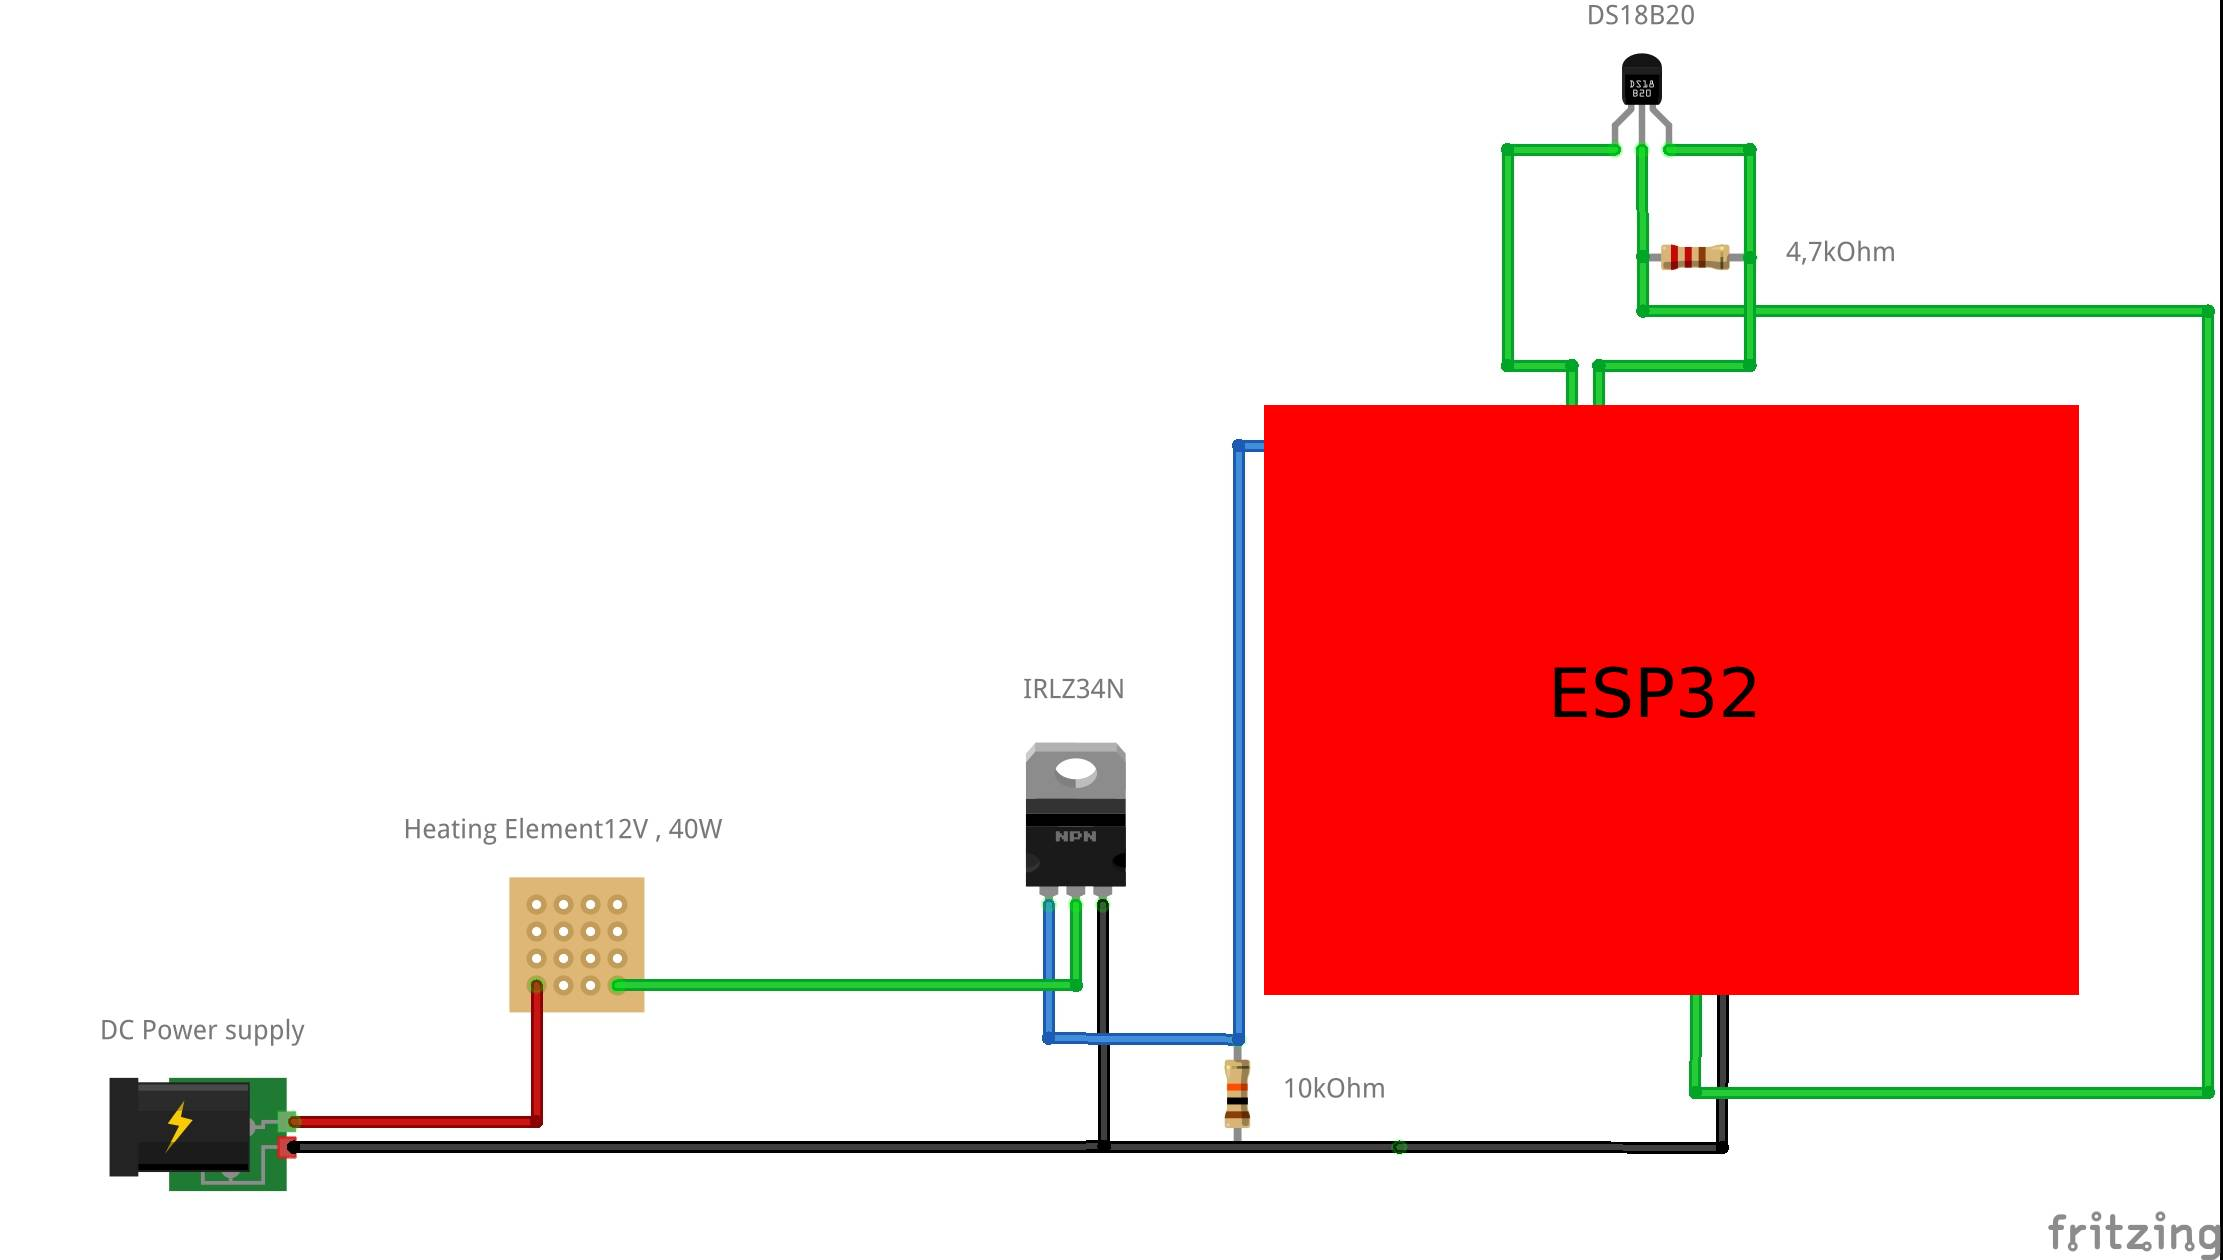
\includegraphics[scale=0.5]{images/temperature_control_diagram.jpg}}
	\caption{Boiling Kettle Temperature Controller Diagram}
\end{figure}

\subsubsection{Source}
This requirement came from Dr. Chris Conly. He requested that our team ensure
that the water stay a constant boiling temperature to maximize extraction.  
\subsubsection{Constraints}
Detailed description of applicable constraints...
\subsubsection{Standards}
\begin{itemize}
\item IEC 60730
\item IEC 60335
\item EN ISO 13849
\end{itemize}
\subsubsection{Priority}
This feature is of \textbf{Critical} priority. Without this feature we would be unable to
accomplish any sort of extraction. 
